\documentclass[10pt]{beamer}

\usetheme[progressbar=frametitle]{metropolis}
\usepackage{appendixnumberbeamer}

\usepackage{booktabs}
\usepackage[scale=2]{ccicons}
\usepackage{braket}
\usepackage{pgfplots}
\usepgfplotslibrary{dateplot}
\usepackage{xspace}

\newcommand{\themename}{\textbf{\textsc{metropolis}}\xspace}
\newcommand{\D}{\mathcal{D}}
\newcommand{\Tr}{\mathrm{Tr}}


\title{Advanced Topics in MBP: Lattice QCD}
\date{29$^\text{th}$ June 2017}
\author{Giovanni Pederiva, Mathias Vege}
\institute{University of Oslo}

\begin{document}

\setbeamercolor{background canvas}{bg=white}
\maketitle

\begin{frame}{Overview}
  \setbeamertemplate{section in toc}[sections numbered]
  \tableofcontents[hideallsubsections]
\end{frame}

\section{Path Integrals: Concepts and Formalism}
\begin{frame}{Path Integrals I}
In the path integral formalism the evolution from a state $\ket{x_i}$ do a state $\ket{x_f}$ from time $t_i$ to time $t_f$ is given by:
\[
	\bra{x_f}e^{-\hat{H}(t_f-t_i)}\ket{x_i} = \int \D x(t) e^{-S[x]}
\]
On the lhs we have the standard quantum mechanical time evolution operator with $\hat{H}$ being the Hamiltonian operator of the system, the rhs represents the path integral of all possible paths x(t) from $x_i$ to $x_f$ with $t = t_i \rightarrow t_f$ weighted with the classical action $S[x]$:
\[
	S[x] = \int_{t_i}^{t_f} dt L(x,\dot{x}) =  \int_{t_i}^{t_f} dt \left( \frac{m\dot{x}(t)^2}{2} - V(x(t))\right)
\]
%% knowledge of the propagator gives full information about the system
\end{frame}

\begin{frame}{Path Integrals II}
In a simple one dimensional case the path integral can be seen as:
\[
	 \int \D x(t) \rightarrow \int_{-\infty}^{\infty} dx_1dx_2\dots dx_{N-1}
\]
where the time has been discretized in N slices from $t_i = t_0$ to $t_f = t_N$. Consequently $x_i = x(t_i)$.  
%% picture??
\end{frame}

\begin{frame}{Computation of Observables}
Given some functional $\Gamma[x]$ that represents an observable at intermediate times of the evolution of the system we can write its expectation value as:
\[
	\braket{\Gamma[x]} = \frac{1}{Z} \int \D x(t) \Gamma[x] e^{-S[x]}
\]
where the normalization $Z$ is given by 
\[
	Z = \int \D x(t) e^{-S[x]}
\]
This can be computed using a set of configurations $x^{(k)} = \{x^{(k)}_1x^{(k)}_2\dots x^{(k)}_{N-1} \}$ for $k = 1,2,\dots N_{cf}$. The Monte Carlo estimator then becomes:
\[
	\braket{\Gamma[x]} \approx \bar{\Gamma} = \frac{1}{N_{cf}} \sum_{k = 1}^k \Gamma[x^{(k)}]
\]
\end{frame}

\begin{frame}{Path Integrals for Field Theories}
When we generalize our theory to a four dimensional euclidean space time an observable that depends on a scalar field can be computed in a very similar fashion as we just described:
\[
	\braket{\Gamma[\phi]} = \frac{1}{Z} \int \D \phi \Gamma[\phi] e^{-S[\phi]}
\]
where the normalization $Z$ is given again by 
\[
	Z = \int \D \phi e^{-S[\phi]}
\]
But this time the path integral can be computed numerically by discretizing the 4 dimensional space in a lattice:
\[
	 \int \D \phi \rightarrow \int \prod_{x_i \in lattice} d\phi(x_i)
\] 
\end{frame}



\section{The Harmonic Oscillator: a Simple Example}
\begin{frame}{The Harmonic Oscillator}
A first example of the path integral solution of quantum mechanical systems can be the 1D Harmonic Oscillator. It is particularly well suited because of:
\begin{itemize}
\item simple dimensional discretization
\item well known results for expectation values
\item fast analytical analysis, implementation and runs 
\end{itemize}
\end{frame}

\begin{frame}{The Harmonic Oscillator}
The classical action for the harmonic oscillator is given by:
\[
	S[x] = \int_{t_i}^{t_f} \left[ \frac{m\dot{x}(t)^2}{2} + \frac{1}{2}\omega x(t)^2\right] dt
\]
We can discretize the time domain into $N$ slices of step $a$, which imposes us to discretize the time derivative of the position as well. When considering the integral between time $t_j$ and $t_{j+1}$ the action becomes:
\[
	S_{j} \approx a\left[ \frac{m(x_{j+1}-x_j)^2}{2a^2} + \frac{1}{4}\omega (x_{j+1} - x_j)^2 \right] dt 
\]
When summing over all time slices (and applying periodic boundary conditions) we get
\[	
	S_{latt} = \sum_{j = 0}^{N-1} \left[ \frac{m}{2a}(x_{j+1}-x_j)^2 + \frac{a}{2} x_j^2 \right]
\]
\end{frame}

\begin{frame}{The Two Point Correlator}
In order to extract information from the system we need to construct and study an observable. We can look at a two point correlator of the form $\langle x(t_2)x(t_1) \rangle$.  
In the continuum this is equivalent to the calculation of the ratio of path integrals:
\[
	\langle x(t_2)x(t_1) \rangle = \frac{\int \D x(t) x(t_2) x(t_1) e^{-S[x]}}{\int \D x(t) e^{-S[x]}}
\]
In quantum mechanics the numerator (using the definition of the path integral) is equal to:
\[	
	\int dx \bra{x} e^{\bar{H}(t_f-t2)} \tilde{x} e^{\bar{H}(t_2-t1)} \tilde{x} e^{\bar{H}(t_1-ti)} \ket{x}
\]
\end{frame}

\begin{frame}{The Two Point Correlator}
If we look at the full integral, let the hamiltionian operator act on the states leaving the spectral decomposition of them, and substitute $T = t_f-Ti$ and $t = t_2 - t_1$ we get to:
\[
	\langle x(t_2)x(t_1) \rangle = \frac{\sum e^{-E_n T} \bra{E_n} \tilde{x} e^{-(\bar{H}-E_n)t}  \tilde{x}\ket{E_n}}{\sum e^{-E_n T }}
\]
and for $T \gg t$ the ground state will dominate the summation:
\[
	G(t) = \langle x(t_2)x(t_1)\rangle \rightarrow  \bra{E_0} \tilde{x} e^{-(\bar{H}-E_0)t}  \tilde{x}\ket{E_0}
\]
and letting $t$ to be large as well the propagator ends up linking the two lowest energy states:
\[
	G(t) \rightarrow  |\bra{E_0} \tilde{x} \ket{E_1}|^2e^{-(E_1-E_0)t}
\]
\end{frame}

\begin{frame}{Discretizing the Two Point Correlator }
We can now extract the first excitation energy of the quantum mechanical harmonic oscillator, in the limit of $t$ large, as:
\[
	\log\left( \frac{G(t)}{G(t+\Delta t)}\right) = (E_1 - E_0)\Delta t
\]
On our discretized lattice the correlator can be obtained numerically by directly computing the average value of the operator:
\[
	G(t) = \frac{1}{N}\sum_j\langle\braket{x(t_j+t)x(t_j)}\rangle
\]
for all $t$ in $0, a, 2a\dots (N-1)a$. This might look trivial at a first glance, but it is the key point of the whole algorithm
\end{frame}

\begin{frame}{The Metropolis Algorithm}
The computational algorithm required to compute the correlator is based on the idea of creating a Markov chain of possible paths for the harmonic oscillator, via subsequent updates. This procedure is called Metropolis algorithm:
\begin{itemize}
\item initialize an array of N position values for each time point (for example set everything to 0)
\item suggest a new random configuration starting from the current one
\item accept or reject the update, based on the action difference
\item compute the correlator for the current configuration
\item repeat the process $N_{cf}$ times, sufficiently large to have a statistically relevant ensemble.
\end{itemize}
\end{frame}


\begin{frame}{Further Details on the Metropolis Algorithm}
\begin{itemize}
\item In order to limit the auto correlation between data, the observable is only computed once every $N_{corr}$ updates. 
\item The rule for accepting an update is: $\exp(-\Delta S) > \xi$. Where $\xi \in [0,1]$, a randomly chosen number. This implies that if the classical action is reduced the update is automatically accepted, if it is positive, a random number $\xi$ is generated and compared with the exponential of the action. This condition allows the system to explore all the phase space and not get stuck in a local minimum for example.
\end{itemize} 
\end{frame}


\begin{frame}{Numerical Tests}
Runs for the HO were made using $10^5$ configurations ($N_{conf}$), skipping 20 updates between every measurement ($N_{corr}$). The time axis was discretized into 20 nodes. Data, to improve the estimate of the error bars, have been resampled using the bootstrap technique. 
The result that is physically relevant is the first excitation energy, which we expect to be $1\hbar\omega$. For simplicity we set $\hbar=\omega=1$ and the lattice spacing parameter $a = 0.5$.
\end{frame}


\begin{frame}{Bootstrapping}
Due to the demanding calculations of LQCD, we implemented statistical bootstrapping. The general method for bootstrapping goes as following: Given a data set of $N$ data points with an observable $\hat{\theta}$. We now \textit{resample} the dataset $K$ times. For each resample, we compute the observable which we call $\theta_k$. We now have $K$ $\theta_k$. We can now compute the average and variance of of the bootstrapped data.
\[
\tilde{\theta} \equiv \frac{1}{K}\sum^K_{k=1}\theta_k,
\]
\[
\sigma^2_{\tilde{\theta}} \equiv \frac{1}{K}\sum^K_{k=1}(\theta_k - \tilde{\theta})^2
\]
\end{frame}


\begin{frame}{Results}
As we can see, the estimate of the energy varies considerably with the correlation time (it is antisymmetric due to periodicity). However it is close to one (or minus one) at both ends. 
\begin{figure}
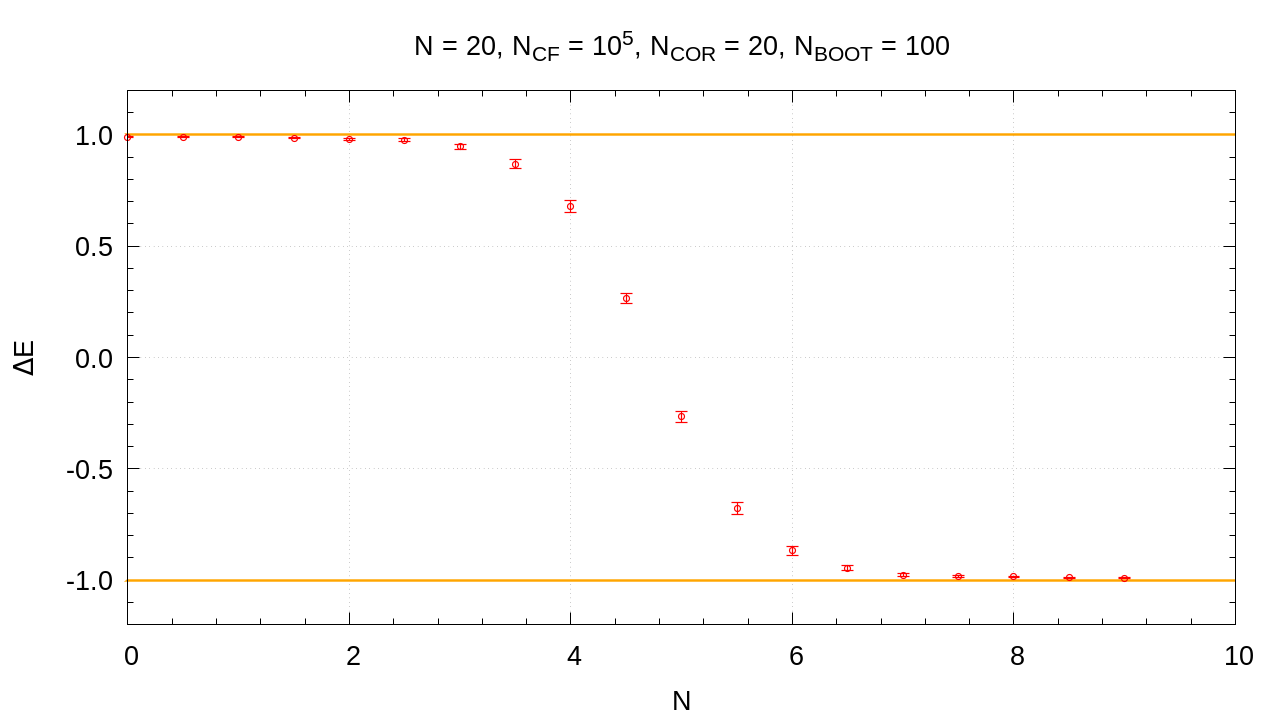
\includegraphics[width=0.8\textwidth]{HOEnergies.png}
\caption{First excitation energy of the harmonic oscillator as a function of the correlation time.}
\end{figure}
\end{frame}


\begin{frame}{Results}
A precise estimate of the excitation energy was obtained by mirroring the last data points to the left of the first ones, and taking a linear fit.
\begin{figure}
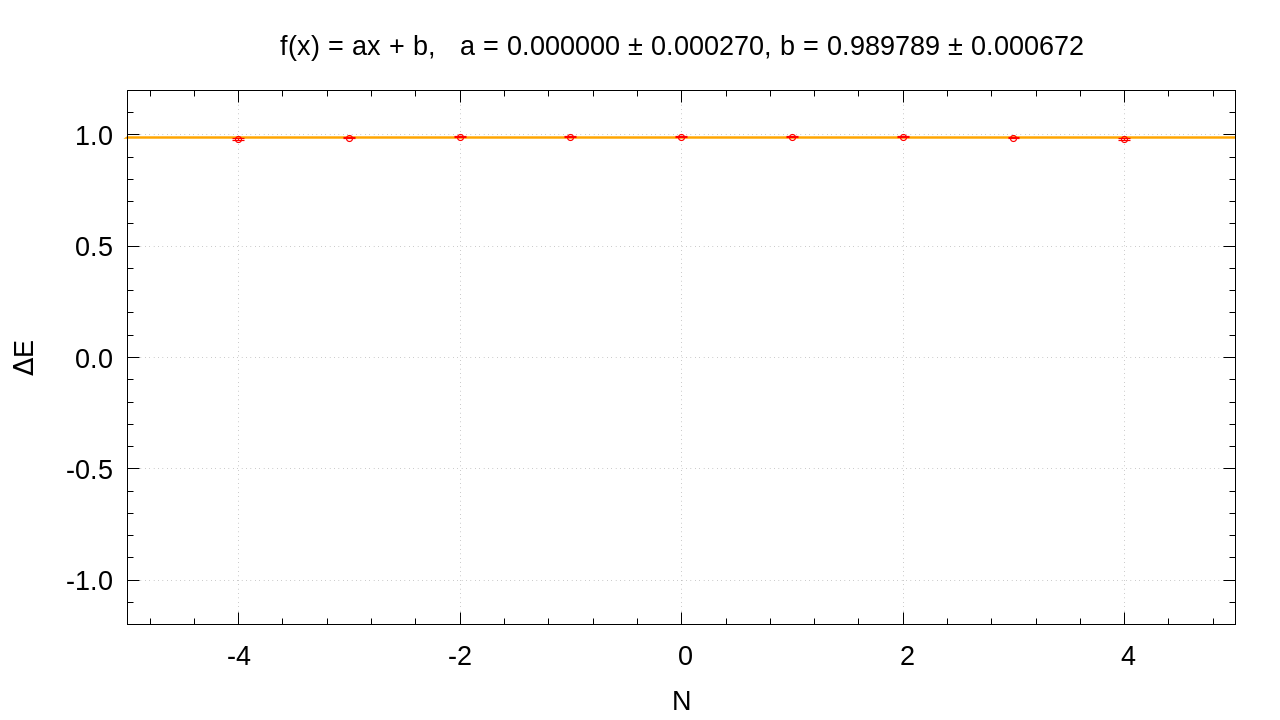
\includegraphics[width=0.8\textwidth]{Fit.png}
\caption{Linear fit results for the first excitation energy of the harmonic oscillator.}
\end{figure}
\end{frame}


\section{Overview of Lattice QCD Calculations}


\begin{frame}{QCD in the continuum}
We are looking at pure gauge action, excluding fermions.
\[
S_G = \int d^4 x \frac{1}{2}\sum_{\mu,\nu}\Tr F_{\mu\nu}^2(x)
\]
with the field strength tensor given as the commutator of the covariant derivatives
\[
F_{\mu\nu}(x) = -i[D_\mu(x,D_\nu(x)]
\]
Our goal is to build a gauge invariant, discretized (gluon) action under the $SU(3)$ gauge symmetry. Demanding invariance under $SU(3)$, forces the covariant derivatives to become,
\[
D_\mu(x) \rightarrow D_\mu'(x) = \partial_\mu+igA'_\mu(x) = \Omega(x) D_\mu(x) \Omega^\dagger(x)
\]
This leads to a more familiar form of the field strength tensor
\[
F_{\mu\nu}(x) = \partial_\mu A_\mu(x) - \partial_\nu A_\mu(x) + ig[A_\mu(x), A_\nu(x)]
\]
with the $g$ being the coupling constant. The $\Omega(x)$ is a $3\times 3$ $SU(3)$ matrix(complex, unitary, $\Omega(x)^\dagger = \Omega(x)^{-1}$ and $\det[\Omega(x)]=1$).
\end{frame}


\begin{frame}{QCD on the lattice I: links}
When translating QCD to the lattice $\Lambda$, we discretize space time to 
\[
\Lambda = \{n=\{n_1,n_2,n_3,n_4\} | n_1,n_2,n_3 = 0,1,\dots,N-1; n_4 =0,1,\dots,N_T-1\}
\]
$N$ is the number of spatial points, and $N_T$ is the temporal ones. A link between two space time points $n$ and $n+\hat{\mu}$ is defined by $SU(3)$ matrices $U_\mu(n)$. The $\hat{\mu}$ indicates a single step in the $\mu$ space time direction. Conversely, going from point $n$ to $n-\hat{\mu}$, is given as (draw on link on blackboard for illustration)
\[
U_{-\mu}(n) \equiv U_{\mu}(n-\hat{\mu})^\dagger
\]
The link, is in this case our gauge field and is given as
\[
U_\mu = \exp(iaA_\mu(n))
\]
This comes from the line integral,
\[
U_\mu(x) = \mathcal{P}\exp\left(-i\int^{x+a\hat{\mu}}_x gA\cdot dx\right) \approx  \exp\left(-igaA_\mu\right)
\]
With the $\mathcal{P}$ being the path ordering of the integral.
\end{frame}


\begin{frame}{QCD on the lattice II: using links to build gauge invariant objects}
We will ignore all other symmetries such as rotational, Lorentz ect., as preserving the gauge symmetry ensures couplings between quark-gluon, three-gluon, four gluons are equal and the bare gluon mass is zero. In order to preserve gauge invariance, we use links to build gauge invariant objects. \textit{All closed loops of connected links are gauge invariant}. The simplest gauge invariant object to build is the \textit{plaquette}(draw on blackboard).
\[
P_{\mu\nu} = U_\mu(n)U_\nu(n+\hat{\mu})U_{-\mu}(n+\hat{\mu}+\hat{\nu})U_{-\nu}(n+\hat{\nu}) 
\]
Using the relation for the inverse gauge link, we can rewrite this to,
\[
P_{\mu\nu} = U_\mu(n)U_\nu(n+\hat{\mu})U_{\mu}(n+\hat{\nu})^\dagger U_{\nu}(n)^\dagger
\]
\end{frame}


\begin{frame}{QCD on the lattice III: Wilson gauge action}
A possible formulation of the discretized gauge action is given by the \textit{Wilson gauge action}.
\[
S_G[U] = \frac{2}{g^2} \sum_x\sum_{\mu <\nu} \mathrm{Re} \Tr [1-P_{\mu\nu}(x)]
\]
No color indices is included, as the trace of the $SU(3)$ matrices ensures that the color is gauge invariant.

It can be shown, that this expression reproduces the continuum action, by using the $\exp(A)\exp(B)=\exp(A+B+\frac{1}{2}[A,B] + \dots)$ for matrices, and the expression for the line integral of $U_\mu(n)$, and then Taylor expanding.
\end{frame}


\begin{frame}{Lattice QCD Calculations}
In general all Lattice QCD Calculations can be designed to be split into two main parts:
\begin{itemize}
\item Generation of Configurations: generating a numerical statistical ensemble of lattice field configurations weighted according to some action. They can be generated through various methods, such as Metropolis algorithm, the Heatbath method or Hybrid Monte Carlo methods. 
\item Computation of Observables: extracting information about correlators, masses, excitation levels from the lattice field configurations. 
\end{itemize}
Usually the ensembles are rather small (few hundreds configurations) so the statistical analysis of observables has to be done using methods as bootstrapping or jackknife.
\end{frame}


\begin{frame}{Observables on the Lattice}
The simplest observable we have is the plaquette operator,
\[
\langle P \rangle = \frac{1}{6|\Lambda|N}\sum_{x,\mu<\nu} \mathrm{Re}\Tr P_{\mu\nu}
\]
with the plaquette being given as earlier,
\[
P_{\mu\nu} = U_\mu(n)U_\nu(n+\hat{\mu})U_{\mu}(n+\hat{\nu})^\dagger U_{\nu}(n)^\dagger
\]
The $|\Lambda|$ is the number of lattice points, $N$ is the number of our gauge group(3 in our case). The 6 stems from us having to average the number of plaquettes we are taking.
\end{frame}


\section{Generating Pure Gauge Field Configurations}
\begin{frame}{Generating Pure Gauge Field Configurations}
Each site on the lattice has 4 $SU(3)$ matrices associated with itself. One for each space time direction. The inverse of this matrix corresponds to the opposite direction. These matrices will be our links $U_\mu(x)$ and represents our gauge field $A_\mu(x)$. In order to generate these matrices, we can do following,
\begin{itemize}
\item We generate random two complex vectors, $\mathbf{u}$ and $\mathbf{v}$
\item We normalize the first column by $|\mathbf{u}|^2=\mathbf{u}^*\cdot \mathbf{u}=1$.
\item Use Gram-Schmitt to make the vectors orthogonal to each other.
\item We normalize the second column.
\item We take the cross product between $\mathbf{u}^* \times \mathbf{v}^*$, to create a third orthonormal column.
\end{itemize}
This proved a possible start configuration for our gauge field. \textit{Problem}: this is a random matrix which is not near the unity, and will make the matrix updates problematic as we may move too far away from the original configuration.
\end{frame}


\begin{frame}{Updating the gauge field I: Metropolis algorithm}
The Metropolis algorithm described in the harmonic oscillator example bear strong resemblance to the one applied for the pure gauge case.  
\begin{itemize}
\item Initialize the lattice to a random $SU(3)$ configuration, or set all matrices to identity.
\item Select one of the links(matrices) at a space time point, and update it by multiplying by a $X$ matrix close to the identity.
\item accept or reject the update, based on the action difference $\Delta S$.
\item compute the correlator for the current configuration
\item repeat this for all links at all space time points.
\end{itemize}
\end{frame}


\begin{frame}{Updating the gauge field II: Change in gauge action}
When computing the change in action for a given updated link $U_\mu'(n)$, we can calculate the following local contribution to the change
\[
\Delta S = - \frac{\beta}{3}\mathrm{Re}\Tr[(U_\mu(n)' - U_\mu(n))A]
\]
where $A$ is the staple product,
\[
\begin{split}
A &= \sum_{\nu\neq\mu}\big( U_\nu(n+\hat{\mu})U_{-\mu}(n+\hat{\mu}+\hat{\nu})U_{-\nu}(n+\hat{\nu}) \\
&+ U_{-\nu}(n+\hat{\mu})U_{-\mu}(n+\hat{\mu}-\hat{\nu})U_{\nu}(n-\hat{\nu})\big)
\end{split}
\]
\end{frame}


\begin{frame}{Updating the gauge field III: the matrix update}
In order to optimize the gauge field updates, we will make the Metropolis update use $SU(3)$ matrices close to the identity.
\[
U_\mu'(n) = X U_\mu(n)
\]
The $X$ matrix will be the a product of three matrices build of matrices containing $SU(2)$ matrices,
\[
X = RST
\]
where R,S and T are built from
\[
R = \begin{pmatrix}
r_{11} & r_{12} & 0 \\
r_{21} & r_{22} & 0 \\
0 & 0 & 1
\end{pmatrix}, 
S = \begin{pmatrix}
s_{11} & 0 & s_{12} \\
0 & 1 & 0 \\
s_{21} & 0 & s_{22}
\end{pmatrix},
T = \begin{pmatrix}
1 & 0 & 0 \\
0 & t_{11} & t_{12} \\
0 & t_{21} & t_{22}
\end{pmatrix}
\]
The $r,s,t$ are $SU(2)$ matrices.
\end{frame}


\begin{frame}{Updating the gauge field IV: further details}
\begin{itemize}
\item As with the HO example, we will in order to limit correlation and computational time only compute the observable once every $N_\text{corr}$ updates.
\item When computing the Wilson gauge action at a point, we will have that the staple $A$ can be computed once for a point, then update that space time point many times in order to save computational time.
\end{itemize}
\end{frame}


\section{Data analysis}
\begin{frame}{Topological susceptibility}
An analysis of the topological susceptibility were performed using the bootstrapping technique. First, the topological susceptibility $\chi_\text{top}$, is related to the topological charge $Q_\text{top}$ which tells us about how many left- and right-handed zero modes.
\begin{figure}
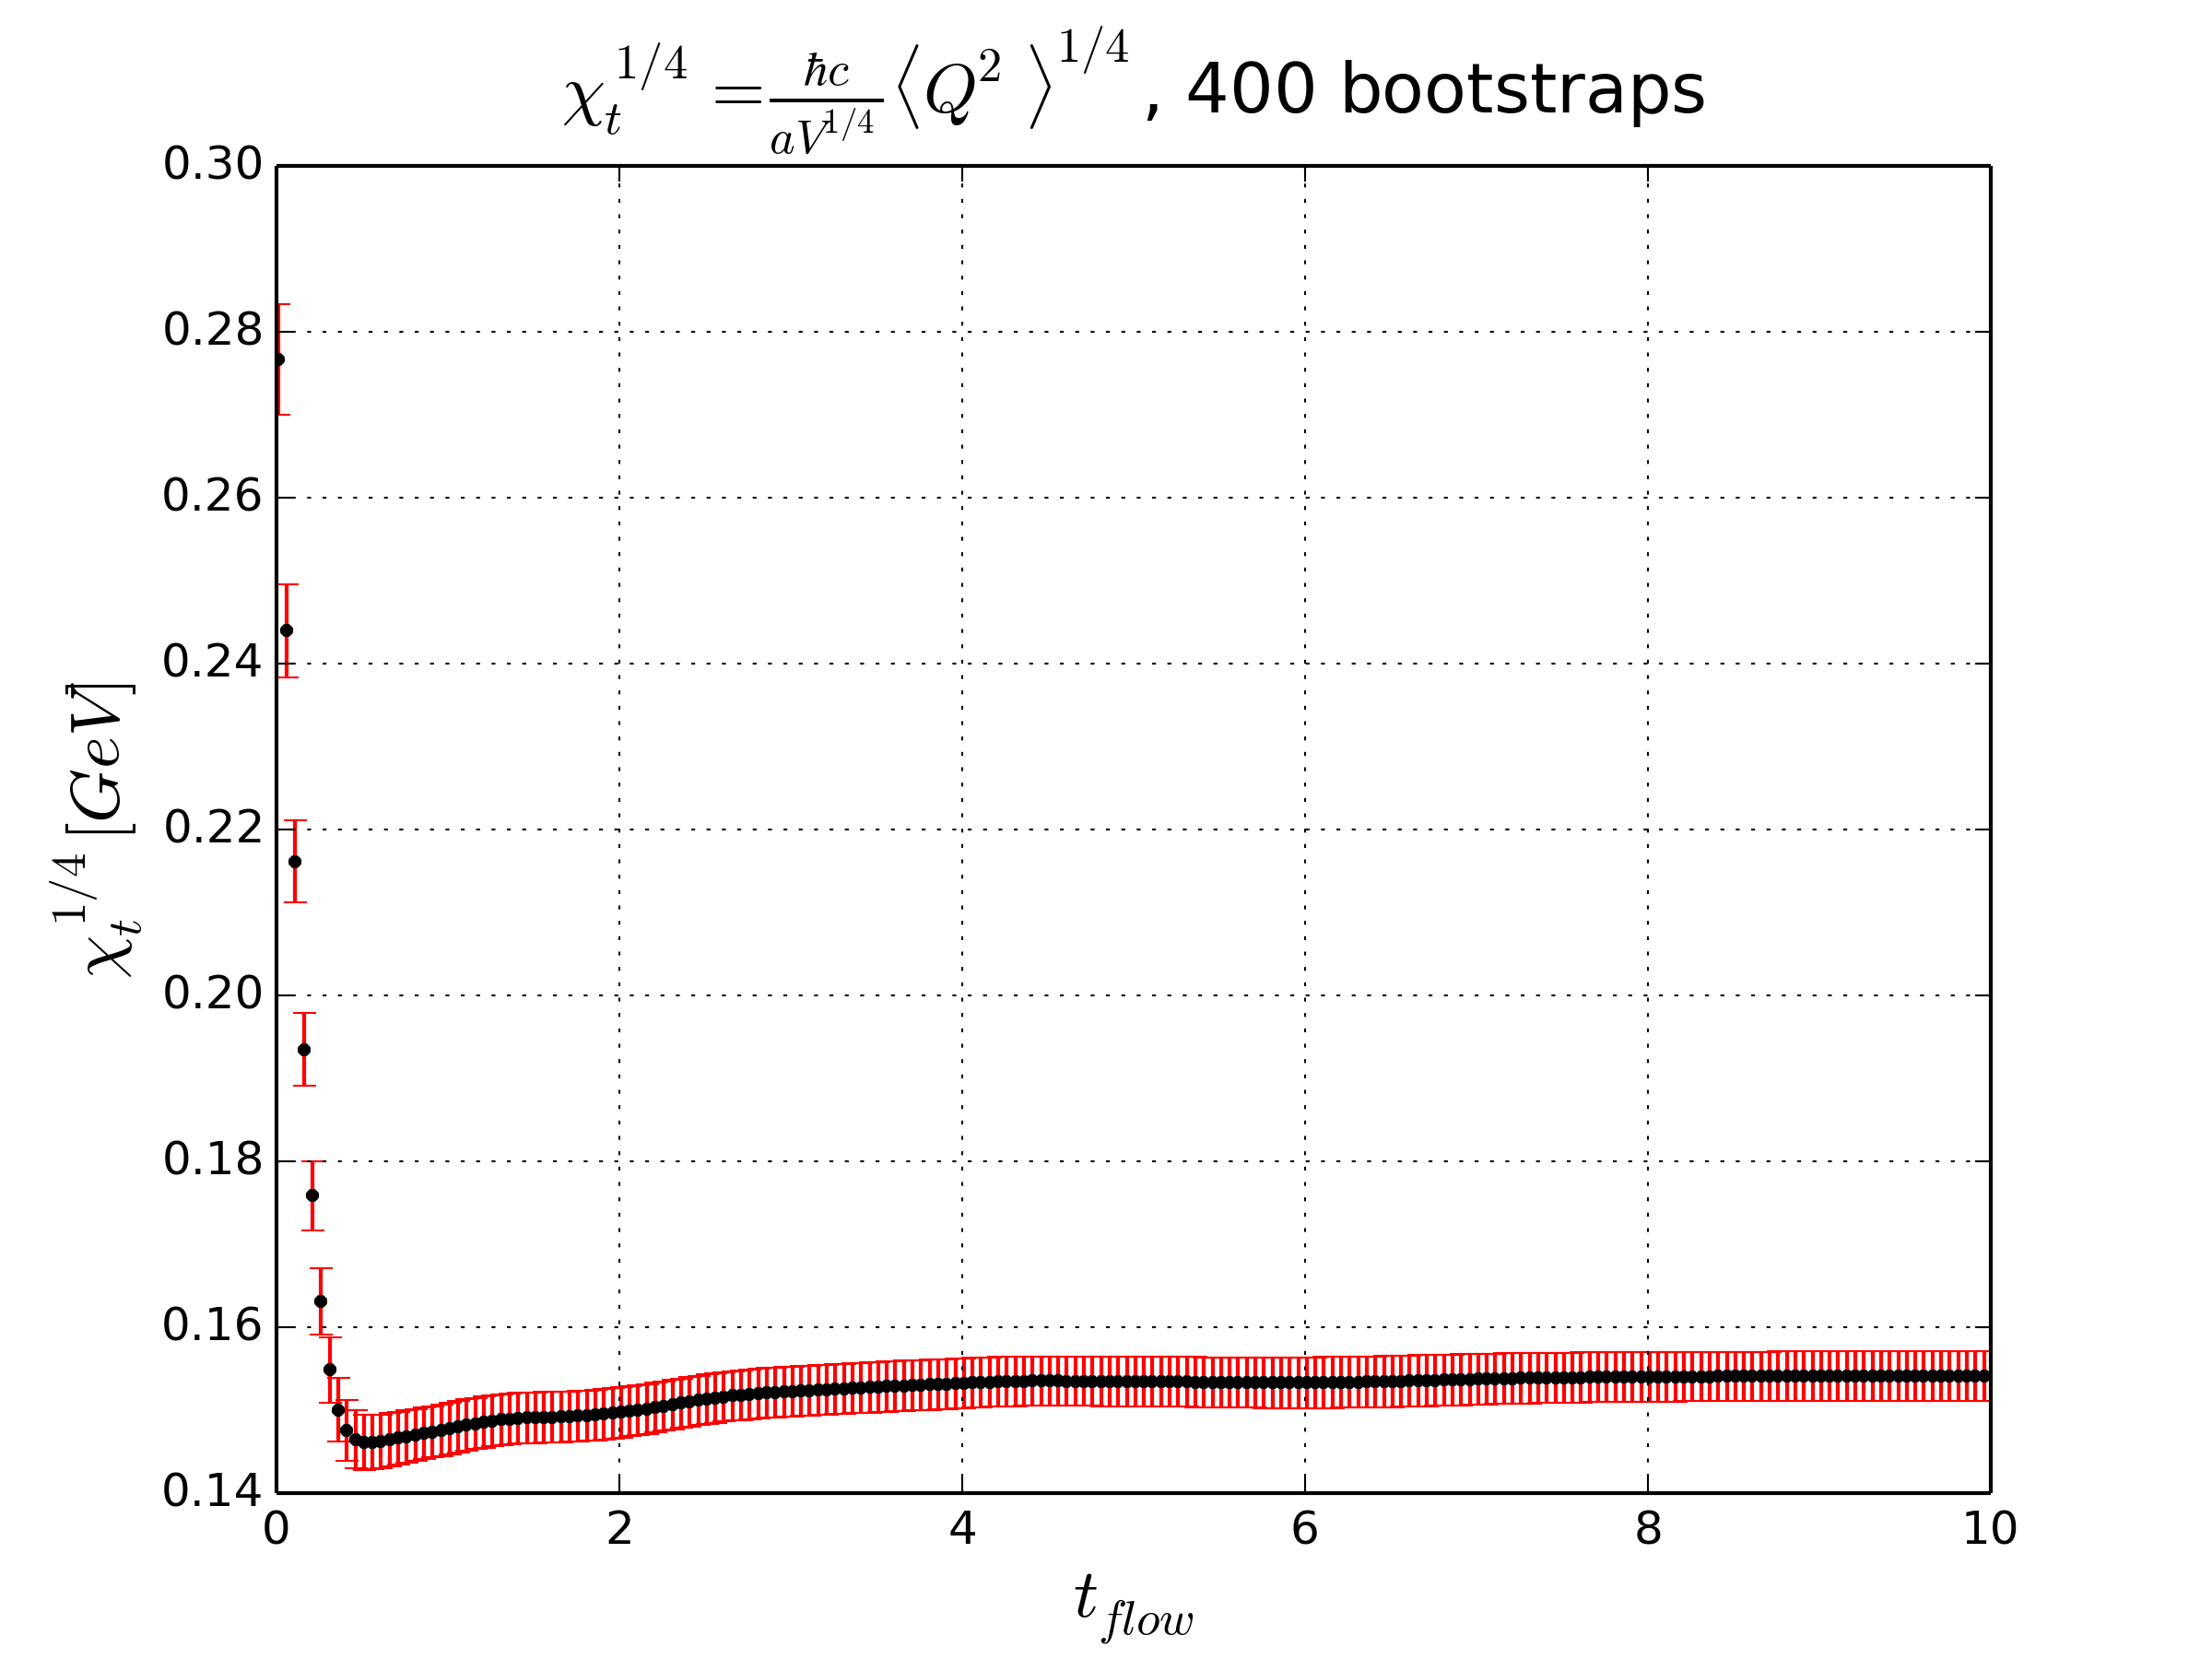
\includegraphics[width=0.65\textwidth]{chi_400bootstraps.png}
\caption{The topological susceptibility with 200 bootstraps.	}
\end{figure}
\end{frame}

\end{document}

